\documentclass[]{elsarticle} %review=doublespace preprint=single 5p=2 column
\usepackage{lmodern}
\usepackage{amssymb,amsmath}
\usepackage{ifxetex,ifluatex}
\usepackage{fixltx2e} % provides \textsubscript
\ifnum 0\ifxetex 1\fi\ifluatex 1\fi=0 % if pdftex
  \usepackage[T1]{fontenc}
  \usepackage[utf8]{inputenc}
\else % if luatex or xelatex
  \ifxetex
    \usepackage{mathspec}
  \else
    \usepackage{fontspec}
  \fi
  \defaultfontfeatures{Ligatures=TeX,Scale=MatchLowercase}
\fi
% use upquote if available, for straight quotes in verbatim environments
\IfFileExists{upquote.sty}{\usepackage{upquote}}{}
% use microtype if available
\IfFileExists{microtype.sty}{%
\usepackage{microtype}
\UseMicrotypeSet[protrusion]{basicmath} % disable protrusion for tt fonts
}{}
\usepackage[margin=1in]{geometry}
\usepackage{hyperref}
\hypersetup{unicode=true,
            pdftitle={Getting Data from the Human Connectome Project (HCP)},
            pdfauthor={John Muschelli},
            pdfborder={0 0 0},
            breaklinks=true}
\urlstyle{same}  % don't use monospace font for urls
\usepackage{color}
\usepackage{fancyvrb}
\newcommand{\VerbBar}{|}
\newcommand{\VERB}{\Verb[commandchars=\\\{\}]}
\DefineVerbatimEnvironment{Highlighting}{Verbatim}{commandchars=\\\{\}}
% Add ',fontsize=\small' for more characters per line
\usepackage{framed}
\definecolor{shadecolor}{RGB}{248,248,248}
\newenvironment{Shaded}{\begin{snugshade}}{\end{snugshade}}
\newcommand{\KeywordTok}[1]{\textcolor[rgb]{0.13,0.29,0.53}{\textbf{{#1}}}}
\newcommand{\DataTypeTok}[1]{\textcolor[rgb]{0.13,0.29,0.53}{{#1}}}
\newcommand{\DecValTok}[1]{\textcolor[rgb]{0.00,0.00,0.81}{{#1}}}
\newcommand{\BaseNTok}[1]{\textcolor[rgb]{0.00,0.00,0.81}{{#1}}}
\newcommand{\FloatTok}[1]{\textcolor[rgb]{0.00,0.00,0.81}{{#1}}}
\newcommand{\ConstantTok}[1]{\textcolor[rgb]{0.00,0.00,0.00}{{#1}}}
\newcommand{\CharTok}[1]{\textcolor[rgb]{0.31,0.60,0.02}{{#1}}}
\newcommand{\SpecialCharTok}[1]{\textcolor[rgb]{0.00,0.00,0.00}{{#1}}}
\newcommand{\StringTok}[1]{\textcolor[rgb]{0.31,0.60,0.02}{{#1}}}
\newcommand{\VerbatimStringTok}[1]{\textcolor[rgb]{0.31,0.60,0.02}{{#1}}}
\newcommand{\SpecialStringTok}[1]{\textcolor[rgb]{0.31,0.60,0.02}{{#1}}}
\newcommand{\ImportTok}[1]{{#1}}
\newcommand{\CommentTok}[1]{\textcolor[rgb]{0.56,0.35,0.01}{\textit{{#1}}}}
\newcommand{\DocumentationTok}[1]{\textcolor[rgb]{0.56,0.35,0.01}{\textbf{\textit{{#1}}}}}
\newcommand{\AnnotationTok}[1]{\textcolor[rgb]{0.56,0.35,0.01}{\textbf{\textit{{#1}}}}}
\newcommand{\CommentVarTok}[1]{\textcolor[rgb]{0.56,0.35,0.01}{\textbf{\textit{{#1}}}}}
\newcommand{\OtherTok}[1]{\textcolor[rgb]{0.56,0.35,0.01}{{#1}}}
\newcommand{\FunctionTok}[1]{\textcolor[rgb]{0.00,0.00,0.00}{{#1}}}
\newcommand{\VariableTok}[1]{\textcolor[rgb]{0.00,0.00,0.00}{{#1}}}
\newcommand{\ControlFlowTok}[1]{\textcolor[rgb]{0.13,0.29,0.53}{\textbf{{#1}}}}
\newcommand{\OperatorTok}[1]{\textcolor[rgb]{0.81,0.36,0.00}{\textbf{{#1}}}}
\newcommand{\BuiltInTok}[1]{{#1}}
\newcommand{\ExtensionTok}[1]{{#1}}
\newcommand{\PreprocessorTok}[1]{\textcolor[rgb]{0.56,0.35,0.01}{\textit{{#1}}}}
\newcommand{\AttributeTok}[1]{\textcolor[rgb]{0.77,0.63,0.00}{{#1}}}
\newcommand{\RegionMarkerTok}[1]{{#1}}
\newcommand{\InformationTok}[1]{\textcolor[rgb]{0.56,0.35,0.01}{\textbf{\textit{{#1}}}}}
\newcommand{\WarningTok}[1]{\textcolor[rgb]{0.56,0.35,0.01}{\textbf{\textit{{#1}}}}}
\newcommand{\AlertTok}[1]{\textcolor[rgb]{0.94,0.16,0.16}{{#1}}}
\newcommand{\ErrorTok}[1]{\textcolor[rgb]{0.64,0.00,0.00}{\textbf{{#1}}}}
\newcommand{\NormalTok}[1]{{#1}}
\usepackage{graphicx,grffile}
\makeatletter
\def\maxwidth{\ifdim\Gin@nat@width>\linewidth\linewidth\else\Gin@nat@width\fi}
\def\maxheight{\ifdim\Gin@nat@height>\textheight\textheight\else\Gin@nat@height\fi}
\makeatother
% Scale images if necessary, so that they will not overflow the page
% margins by default, and it is still possible to overwrite the defaults
% using explicit options in \includegraphics[width, height, ...]{}
\setkeys{Gin}{width=\maxwidth,height=\maxheight,keepaspectratio}
\IfFileExists{parskip.sty}{%
\usepackage{parskip}
}{% else
\setlength{\parindent}{0pt}
\setlength{\parskip}{6pt plus 2pt minus 1pt}
}
\setlength{\emergencystretch}{3em}  % prevent overfull lines
\providecommand{\tightlist}{%
  \setlength{\itemsep}{0pt}\setlength{\parskip}{0pt}}
\setcounter{secnumdepth}{0}
% Redefines (sub)paragraphs to behave more like sections
\ifx\paragraph\undefined\else
\let\oldparagraph\paragraph
\renewcommand{\paragraph}[1]{\oldparagraph{#1}\mbox{}}
\fi
\ifx\subparagraph\undefined\else
\let\oldsubparagraph\subparagraph
\renewcommand{\subparagraph}[1]{\oldsubparagraph{#1}\mbox{}}
\fi

%%% Use protect on footnotes to avoid problems with footnotes in titles
\let\rmarkdownfootnote\footnote%
\def\footnote{\protect\rmarkdownfootnote}

%%% Change title format to be more compact
\usepackage{titling}

% Create subtitle command for use in maketitle
\newcommand{\subtitle}[1]{
  \posttitle{
    \begin{center}\large#1\end{center}
    }
}

\setlength{\droptitle}{-2em}
  \title{Getting Data from the Human Connectome Project (HCP)}
  \pretitle{\vspace{\droptitle}\centering\huge}
  \posttitle{\par}
  \author{John Muschelli}
  \preauthor{\centering\large\emph}
  \postauthor{\par}
  \predate{\centering\large\emph}
  \postdate{\par}
  \date{2016-11-18}

%%% Begin My package additions %%%%%%%%%%%%%%%%%%%
\usepackage[hyphens]{url}
\usepackage{lineno} % add
\providecommand{\tightlist}{%
  \setlength{\itemsep}{0pt}\setlength{\parskip}{0pt}}
\usepackage{graphicx}
\usepackage{booktabs} 
\usepackage{float}
\usepackage{xcolor}
\usepackage{color}


\usepackage{caption}
\captionsetup{belowskip=20pt,aboveskip=4pt}


% A modified page layout
\textwidth 6.75in
\oddsidemargin -0.15in
\evensidemargin -0.15in
\textheight 9in
\topmargin -0.5in
%%%%%%%%%%%%%%%% end my additions to header

\usepackage[T1]{fontenc}
\usepackage{lmodern}
\usepackage{amssymb,amsmath}
\usepackage{ifxetex,ifluatex}
% use upquote if available, for straight quotes in verbatim environments
\IfFileExists{upquote.sty}{\usepackage{upquote}}{}
\ifnum 0\ifxetex 1\fi\ifluatex 1\fi=0 % if pdftex
  \usepackage[utf8]{inputenc}
\else % if luatex or xelatex
  \usepackage{fontspec}
  \ifxetex
    \usepackage{xltxtra,xunicode}
  \fi
  \defaultfontfeatures{Mapping=tex-text,Scale=MatchLowercase}
  \newcommand{\euro}{€}
\fi
% use microtype if available
\IfFileExists{microtype.sty}{\usepackage{microtype}}{}
\ifxetex
  \usepackage[setpagesize=false, % page size defined by xetex
              unicode=false, % unicode breaks when used with xetex
              xetex]{hyperref}
\else
  \usepackage[unicode=true]{hyperref}
\fi
\hypersetup{breaklinks=true,
            pdfauthor={},
            pdftitle={Neuroconductor: A Framework for Reproducible Neuroimaging Analysis in R},
            colorlinks=true,
            urlcolor=blue,
            linkcolor=magenta,
            pdfborder={0 0 0}}
\urlstyle{same}  % don't use monospace font for urls
\setlength{\parindent}{0pt}
\setlength{\parskip}{6pt plus 2pt minus 1pt}
\setlength{\emergencystretch}{3em}  % prevent overfull lines
\setcounter{secnumdepth}{0}
% Pandoc toggle for numbering sections (defaults to be off)
\setcounter{secnumdepth}{0}
% Pandoc header

%%% John commands standardized
\newcommand{\code}[1]{\texttt{#1}}
\newcommand{\pkg}[1]{\emph{#1}}
\newcommand{\rlang}{\texttt{R}}



\usepackage[nomarkers]{endfloat}
\newcommand{\fixme}[1]{{\color{red} #1}}
\begin{document}
\begin{frontmatter}

  \title{Neuroconductor: An R platform for Neuroimaging}
    \author[JHU]{John Muschelli\corref{c1}}
   \ead{jmusche1@jhu.edu} 
   \cortext[c1]{Corresponding Author}
    \author[Penn]{Jean-Philippe Fortin}
   \ead{fortin946@gmail.com} 
  
    \author[JHU]{Adrian Gherman}
   \ead{adig@jhu.edu} 
   \author[Biogen]{Brian Avants}
   \ead{stnava@gmail.com}
   
   \author[Klarismo,Imperial]{Brandon Whitcher}
   \ead{bwhitcher@gmail.com}   
   
    \author[JHU]{Brian S. Caffo}
   \ead{bcaffo@jhsph.edu} 
  
    \author[JHU]{Ciprian M. Crainiceanu}
   \ead{ccraini1@jhu.edu} 
  
      \address[JHU]{Johns Hopkins Bloomberg School of Public Health, Department of
Biostatistics, 615 N Wolfe St, Baltimore, MD, 21205}
    \address[Penn]{Perelman School of Medicine, University of Pennsylvania, Department of
Biostatistics and Epidemiology, 423 Guardian Drive, Philadelphia, PA
19104}
      \address[Biogen]{Biogen, Cambridge, MA 02142}
      \address[Klarismo]{Klarismo Ltd, London, UK}
      \address[Imperial]{Department of Mathematics, Imperial College London, London, UK}
  
  \begin{abstract}
Neuroconductor (\url{https://neuroconductor.org}) is an open-source platform for rapid testing and dissemination of reproducible computational imaging software. The goals of the project are to: 1) provide a centralized repository of R software dedicated to image analysis, 2) disseminate  software updates quickly, 3) train a large, diverse community of scientists using detailed tutorials and short courses, 4) increase software quality via automatic and manual quality controls, and 5) promote reproducibility of image data analysis. Based on the  programming language R (\url{https://cran.r-project.org/}), Neuroconductor starts with 24 inter-operable packages that cover multiple areas of imaging including visualization, data processing and storage, and statistical inference. Neuroconductor accepts new R package submissions, which are subject to a formal review and continuous automated testing. We provide a description of Neuroconductor's purpose and the user and developer experience.  
\end{abstract}
 
 \end{frontmatter}

% Introduction
\section{Introduction}\label{introduction}

Neuroimaging software is heterogeneous, complex, and hard to use in fully reproducible analytic pipelines. These problems have been accentuated by the diversity of new imaging datasets and associated scientific problems. Indeed, many studies now collect data on thousands of subjects, at multiple visits, and different modalities. Storing, understanding, and analyzing such data is  daunting.  Neuroconductor will provide the software tools for using, improving and designing open source scripted software that depends on a minimum number of software platforms and is dedicated to improving the correctness, reproducibility, and speed of neuroimaging data analysis. To achieve this, Neuroconductor will interweave pre- and post-processing image analysis and will provide integrated data analytic approaches.


Neuroconductor provides data, methods, and software packages designed to support the analysis of image population studies in R (\url{https://cran.r-project.org/}), a programming language with state-of-the-art statistical analysis tools. Neuroconductor supports many types of imaging data including magnetic resonance imaging (MRI: structural, functional, and dynamic), computed tomography (CT), single-photon and positron emission computed tomography, (SPECT and PET), and magnetoencephalography (MEG). It is currently focused on human imaging, especially of the brain; but, it supports other biological imaging.  Neuroconductor can interface with mature R distribution platforms, such as Bioconductor \cite{bioc1,bioc2} and CRAN \cite{Hornik2016,r}.  Although these other distribution platforms exist, we believe that Neuroconductor can enable better support and testing for imaging-specific packages, similar to how Bioconductor supports bioinformatics packages.  
% why not cran?

Neuroconductor can be used seamlessly for data fusion analyses where imaging, genomics, and other types of high-throughput data types are analyzed together with traditional measurements and health outcomes. In R these analyses can be integrated with well designed and tested analytic packages for visualization, inference, longitudinal and survival analysis, regression, network analysis, and machine learning.


\section{The user perspective}\label{section:user_perspective}
The Neuroconductor users interact with the platform via the Neuroconductor website (\url{https://neuroconductor.org}). Users can install an R package, explore packages, or identify a workflow designed for their specific problem. If the workflow does not exist in Neuroconductor then users can create and submit their own. 


\subsection{General description}\label{subsec:general_description}
To download a package a user needs to know the package name, which can be obtained from the \href{list of packages}{https://neuroconductor.org/list-current-packages} on the Neuroconductor webpage. For example, to download the \pkg{fslr} and \pkg{hcp} packages in R the command line instructions are: 

\color{blue}
\begin{verbatim}
source("https://neuroconductor.org/neurocLite.R") 
neuro_install(c("fslr", "hcp"))
\end{verbatim}
\color{black}

Each package contains documentation as vignettes and manuals. Large areas of research covering multiple package combinations are described under Training. Some of these areas contain tutorials and Massive  Open Online Courses (MOOCs) that provide a rapid introduction of more complex concepts and workflows. Examples of such courses are Principles of fMRI  (\url{https://www.coursera.org/learn/functional-mri}) and Introduction to Neurohacking in R (\url{https://www.coursera.org/learn/neurohacking}).  If the user does not find what they are looking for, they can request a tutorial on a specific topic and developers can also submit their own tutorial or course to Neuroconductor. Furthermore, the user can turn to the Support forum,  can attend short courses, take free online MOOCs, or read tutorials. All package developers are users and some users become package developers.

The user may have their own data, use a data package from Neuroconductor, or use a Neuroconductor package  to download data from an internet repository.  
After obtaining data, a first step is to manipulate, visualize, and quality control it.  Most quality control procedures can be performed at the image or subject level, though the distribution of quality metrics in the population can be used as well; see Mejia et al. \citep{mejia2015pca} for an example. Once data quality has been assessed, an analytic database of subjects for subsequent analyses can be created.   

A major advantage of the R environment is that analyses can take advantage of a large collection of well tested,  state-of-the-art statistical packages. For example, using demographic information, regression, mixed effects models, or survival analysis is straightforward in R.  Moreover, the \pkg{voxel} package implements most of these method at a voxel level directly on images \citep{voxel}.  Results containing spatial information can be mapped back to an image, while other results can be displayed using plotting packages such as \pkg{ggplot2} \citep{ggplot2}.  All these steps can be wrapped in a series of reproducible reports using \pkg{knitr} and \pkg{rmarkdown} \citep{rmarkdown,knitr}. Another advantage of R is that complex processing steps and complete analyses can be wrapped into R packages. For example, the \pkg{ichseg} \cite{ichseg,muschelli2016pitch} {\rlang} package is designed for intra-cranial hemorrhage segmentation and it is a wrapper for multiple functions. It uses a  single CT scan as input, processes the data using FSL \citep{fsl}, called through \pkg{fslr} in R \citep{fslr}, and creates a segmentation of the hemorrhagic stroke based on a pre-trained supervised machine learning algorithm. Last, data products resulting from analysis and package development can be deployed as Shiny applications \citep{shiny}, which are web applications built in R and can be accessed with internet browsers.  Shiny applications can be hosted on a user's custom launched or commercial Shiny server (such as \url{www.shinyapps.io}). Below we provide several case studies to build up the intuition for interfacing with  Neuroconductor.

% Case study
\subsection{Case study: structural magnetic resonance imaging processing} Figure~\ref{fig:flow} provides an example of a typical processing pipeline for multi-sequence MRI data. Analysis of such data often begins with a conversion of Digital Imaging and Communications in Medicine (DICOM) files, which are essentially JPEG images with header information.  DICOM is one of the most common formats for imaging data that come directly from the imaging device.  These DICOM files are converted to the Neuroimaging Informatics Technology Initiative (NIfTI) format, one of the most common neuroimaging formats. This process can be done in {\rlang} using the \pkg{dcm2niir} package \citep{dcm2niir}, which calls \texttt{dcm2niix} (\url{https://www.nitrc.org/projects/mricrogl/}), or the \pkg{oro.dicom} \cite{oro.nifti} package. The resulting NIfTI files can be converted to array-based S4 objects  using the \pkg{oro.nifti} \cite{oro.nifti} package or objects based on C++ pointers using the \pkg{ANTsR} \cite{antsr} and \pkg{RNifti} \cite{Rnifti} packages.  These packages also provide the ability to read other neuroimaging formats, such as ANALYZE or NRRD formats.
 
% Flow chart John
\begin{figure}[!ht]
  \begin{center}
    \caption{Typical processing pipeline for multi-sequence structural MRI data.}
    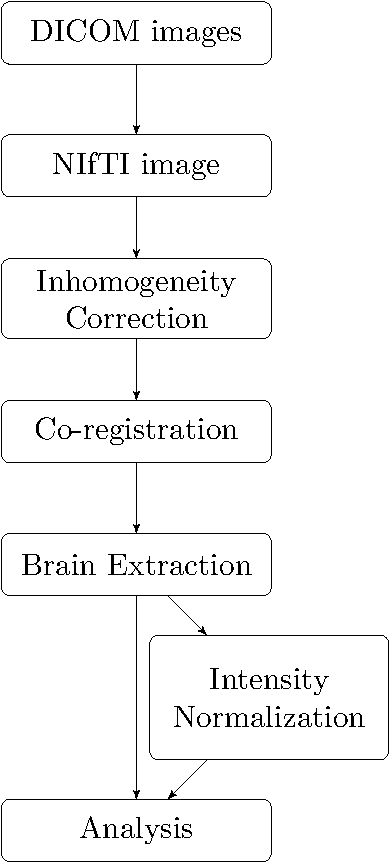
\includegraphics{figures/Imaging_Pipeline_Flowchart.pdf}
    \label{fig:flow}
  \end{center}
\end{figure}


After conversion, image intensity inhomogeneity correction can be applied to ensure that each tissue has similar intensity distributions across locations in the brain (e.g. top versus bottom of the brain). Image inhomogeneities are typically caused by magnetic field inhomogeneities and can be handled by multiple methods. Neuroconductor currently contains 4 such methods implemented in FSL via \pkg{fslr} \cite{zhang_segmentation_2001},  \pkg{freesurfer} \cite{sled_nonparametric_1998}, and \pkg{ANTsR} (N3 and N4 correction) \cite{sled_nonparametric_1998,tustison_n4itk:_2010}.  The next step is co-registration, the process that spatially realigns all images in the sequence to one of the images in the sequence, usually a T1-weighted (T1w) image.  Co-registration can be done using \code{flirt} (\pkg{fslr}), \code{antsRegistration} (\pkg{ANTsR}), or \code{dramms} (\pkg{drammsr}) \cite{dramms}. Co-registration is followed by brain extraction, also known as skull stripping.  This procedure is commonly done on the T1w image, and can be implemented using \pkg{spm12r}, \pkg{fslr}, \pkg{freesurfer}, or \pkg{ANTsR}. At this point, the image sequences for the patient are in the same space and extracranial tissues have been removed.

Brain extraction can be followed by intensity normalization,  which transform the arbitrary units in MRI into interpretable units across subjects. This is not usually thought of as a standard preprocessing step, but it is crucial in many applications. For example, one could be interested in subtracting two images that were collected longitudinally to identify changes or one may want to investigate changes in voxel or ROI intensities over time.  This can be done using z-scoring with respect to a particular tissue class as implemented in WhiteStripe (\pkg{WhiteStripe}) \citep{whitestripe}, standard and robust z-scoring relative to whole brain (\pkg{neurobase}), histogram matching (implemented in \pkg{RAVEL}), or removal of unwanted variation (\pkg{RAVEL}) \citep{ravel}.  Further subject-specific and population analyses may require registration to a population-level template and/or tissue class segmentation. Both these approaches can be done using Nonconductor packages including \pkg{spm12r}, \pkg{fslr}, and \pkg{ANTsR}.

While the flowchart in Figure~\ref{fig:flow} provides a conceptual pre-processing pipeline, deploying an explicit and reproducible pipeline requires specific choices at every step that may depend on multiple tuning parameters. In {\rlang} one can be explicit about these choices, provide a software suite of packages and tuning parameters, and quickly compare results based on different combinations of software and platforms.  

% Example of a cross-package Neuroconductor workflow: preprocessing and analysis of diffusion tensor imaging data
\section{Example of a cross-package Neuroconductor workflow: preprocessing and analysis of diffusion tensor imaging data}

In this section, we discuss an example of complete analysis (preprocessing and statistical analysis) performed entirely within Neuroconductor.  We start with a simple question: in a population of healthy subjects, is there any difference in the white matter (WM) microstructure between males and females? Diffusion tensor imaging (DTI) has been  used extensively to study WM fiber structure by taking advantage of the differential water diffusivity in the WM tracts relative to other brain structures. Fractional anisotropy (FA) and mean diffusivity (MD) are two scalar maps commonly derived from DTI images to study the diffusivity properties of the brain. FA measures the degree of directional diffusivity in a voxel and MD measures the total diffusion within a voxel \cite{fa}.

To investigate potential gender differences in WM fiber tracts, we use DTI images from healthy young adults from The Human Connectome Project (HCP), available at (\url{http://db.humanconnectome.org}).  HCP includes a large cohort of individuals ($N > 1200$) with a vast amount of neuroimaging data, including structural magnetic resonance imaging (sMRI), task and resting state functional MRI (fMRI) and diffusion tensor imaging (DTI).

% Step 1: Downloading data from the hcp package
\subsection{Step 1: Downloading data using the \pkg{hcp} package}
The first step is to download the minimally preprocessed DTI data \citep{hcpminimal} and structural T1w MRI images, available  for 781 subjects (436 females and 345 males), using the \pkg{hcp} \citep{hcp} package.  The \pkg{hcp} package is an \rlang~interface for downloading data from the HCP database, which is publicly available from Amazon Web Services (AWS). A description of how to connect to the HCP database via AWS can be found \href{https://wiki.humanconnectome.org/display/PublicData/How+To+Connect+to+Connectome+Data+via+AWS}{here}.  After accepting the data use terms, one needs to obtain AWS credentials, which include an access key identifier and a secret  key. The \pkg{hcp} package in {\rlang} accesses the data from an Amazon Simple Storage Solution (S3) bucket using these two AWS access keys.  We can set these keys using \code{set\_aws\_api\_key}:
\color{blue}
\begin{verbatim}
library(hcp)
set_aws_api_key(access_key = "ACCESS_KEY", secret_key = "SECRET_KEY")
\end{verbatim}
\color{black}
For instance, the complete diffusion data directory for subject 100307 can be downloaded using the \code{download\_hcp\_dir} function in the \pkg{hcp} package:
\color{blue}
\begin{verbatim}
result <- download_hcp_dir("HCP/100307/T1w/Diffusion")
\end{verbatim}
\color{black}
The \code{result} is an {\rlang}m list containing the file names of all downloaded files, the directory where the files were downloaded, and the \texttt{http} request that was sent to the Amazon S3 bucket. Data from other subjects can be downloaded similarly. After the minimally processed DTI data are downloaded, it can be further processed using \pkg{rcamino}. 

% Step 2: Processing data with rcamino
\subsubsection{Step 2: Processing DTI data with rcamino}

We process the DTI data using the Neuroconductor package \pkg{rcamino}, an \rlang~interface for the open-source DTI software \texttt{Camino} \citep{camino}. The package is used to create and fit the diffusion tensor models, and generate the FA and MD maps. We show below the associated \rlang~code. 

\color{blue}
\begin{verbatim}
# Extract the DTI files for the subject and name them using the NIfTI format
library(neurobase)
library(rcamino)
outfiles <- result$output_files
names(outfiles) <- neurobase::nii.stub(basename(outfiles))

# Specify the B-values and B-vectors used in the HCP database for further processing:
camino_fsl2scheme(bvecs = outfiles[["bvecs"]], bvals = outfiles[["bvals"]],
    outfile = "hcp.scheme")

# Convert the diffusion data from NIfTI to Camino format:
camino_image2voxel(infile = outfiles[["data"]], outfile = "dwi.Bfloat")

# Fit the diffusion tensor imaging model:
camino_modelfit(infile = "dwi.Bfloat", outfile = "dt.Bdouble", 
    scheme = "hcp.scheme", gradadj = outfiles[["grad_dev"]],
    model = "ldt", mask = outfiles[["nodif_brain_mask"]])

# Produce the FA and MD maps from the fitted tensor data:
fa <- camino_fa_img(infile = "dt.Bdouble", inputmodel = "dt", header = outfiles[["data"]])
md <- camino_md_img(infile = "dt.Bdouble", inputmodel = "dt", header = outfiles[["data"]])
\end{verbatim}
\color{black}
Note that \texttt{Camino} requires the b-values and b-vectors of the DTI to conduct the DTI model fit. The B-values are the amount of diffusion weighting used for each volume. The B-vectors are the gradient directions used by the scanner that may depend on the number of directions; for more details, see \url{http://www.diffusion-imaging.com/2014/03/dti-quality-control-part-2-tensor.html}. The process is then repeated for all subjects with available DTI data, and can be sped up by parallel computing.

% Step 3: joint analysis
\subsubsection{Step 3: Nonlinear registration to template} 
The next step is to prepare the data for voxel-wise analysis, which requires the FA and MD maps to be spatially registered to a common template. For each subject, we use the \code{download\_hcp\_file} function from the \pkg{hcp} package to download the T1w image with extra-cranial voxels removed. We then use the diffeomorphic non-linear registration implemented in \pkg{ANTsR}, wrapped in \pkg{extrantsr}, to register FA and MD maps to the 1mm isotropic Eve template T1w image \citep{eve}. The Eve template is a single-subject template created by the Laboratory of Brain Anatomical MRI led by Professor Susumu Mori at Johns Hopkins University. The Eve template is made available in the Neuroconductor data package \pkg{EveTemplate} \cite{eve, MNITemplate}. Alternatively, one could register  images to the MNI template, which is available in the Neuroconductor data package \pkg{MNITemplate} \cite{mni,MNITemplate}.   Each registered DTI map is saved as a standard NIfTI file for further analyses. The \rlang~code is presented below.

\color{blue}
\begin{verbatim}
# Specify the path of the Eve template file:
library(EveTemplate)
eve_template = getEvePath()

# Perform non-linear registration usin Syn in ANTsR:
t1_file <- download_hcp_file("HCP/100307/T1w/T1w_acpc_dc_restore_brain.nii.gz")
reg <- extrantsr::registration(filename = t1_file,  template.file = eve_template, 
    typeofTransform = "SyN", interpolator = "Linear", remove.warp = FALSE)

# Create the registered FA and MD maps to the Eve atlas:
fa_eve <- ants_apply_transforms(fixed = eve_template, moving = fa, 
    transformlist = reg$fwdtransforms)
md_eve <- ants_apply_transforms(fixed = eve_template, moving = md,
    transformlist = reg$fwdtransforms)    
\end{verbatim}
\color{black}

The results of these processing steps are images containing the FA and MD maps registered to the Eve atlas for every subject. While at this point we do not conduct region of interest (ROI) analyses, the template would be useful to extract subject-specific ROIs. An ROI could be defined as an anatomical region, regions obtained from other analyses, or regions that are manually delineated. Here, we focus on voxel-wise analysis across subjects, which can be done because images are registered to a common template space.  Although we do not present any measures of quality control or registration accuracy, users should inspect registration and image quality, either by automated methods or visual inspection.
% discuss Reg errors/QC?

% Step 4: statistical analysis
\subsubsection{Step 4: Statistical analysis} 
The next step is the analysis of the population of images using statistical inference. Neuroimaging convention refers to this step as ``statistical analysis'', a convention we adopt here, despite the fact that the earlier steps clearly involve a great deal of statistical analysis.

We first read the registered NIfTI files into \rlang~and create a matrix of voxels intensities with voxels as rows, and subjects as columns. For the analysis, we only consider voxels in the WM and GM. We create one matrix for the FA maps, and one for the MD maps, using the function \code{images2matrix} from the package \pkg{neurobase}. The registered-to-Eve images for all subjects are located in the lists \code{files.fa} and \code{files.md} for FA and MD maps, respectively. For brevity, we present only the analysis for the MD maps.  In this example, the matrix (\code{Y.md}) has $1,372,619$ rows (number of GM and WM voxels in the Eve template) and $781$ columns (number of subjects in the dataset):
\color{blue}
\begin{verbatim}
# Create the GM and WM mask in Eve template space:
mask <- readEveSeg()

# Discard voxels in the CSF
mask[mask ==1] <- 0 

# All voxels in GM (label = 2) and WM (label =3) are kept
mask[mask %in% c(2,3)] <- 1

# Create the matrix for MD values at every voxel in the mask
Y.md <- images2matrix(files.md, mask=mask)
\end{verbatim}
\color{black}


There are many options in {\rlang} to quantify the association of the FA and MD intensities with gender. The simplest approach is to calculate mass-univariate two-sample t-statistics (t-statistics computed at each voxel separately), which can be quickly computed using \pkg{limma} \citep{limma1,limma2, limma3}, a popular R package from the Bioconductor project (\url{https://www.bioconductor.org/}). The package was originally developed for the analysis of high-throughput genomics data, but much of its functionality can be used in neuroimaging applications without additional effort. Among other methods, the \pkg{limma} package implements Empirical-Bayes (EB) methods to estimate t-statistics based on variance shrinkage (called moderated t-statistics). Below, we present the code to compute the moderated t-statistics for the association between gender and MD, adjusted for age. 

\color{blue}
\begin{verbatim}
# Fit the EB linear model with limma:
library(limma)
fit.md <- eBayes(lmFit(Y.md, model.matrix(~gender+age)))

# Get moderated t-statistics for gender:
t.md    <- fit.md$t[,2]

# Store the moderated t-statistics into template space:
img.t.md <- remake_img(t.md, img=mask, mask=mask)
\end{verbatim}
\color{black}

The code produces t-statistics comparing males versus females in the Eve-template space.  Below, we investigate where the largest differences are located. 

% Step 5: Visualization of the results
\subsubsection{Step 5: Visualization and localization of the results}

A considerable advantage of the close integration between pre- and post-processing tools is that results can be easily mapped back into the native or template space. This can help localize significant associations using template labels. For example, we can identify the voxels that exhibit the largest differences between males and females using the Eve white matter parcellation map (WMPM) \citep{eve}, included in the package \pkg{EveTemplate}. Below, we provide the {\rlang}  code for localization of these results.

\color{blue}
\begin{verbatim}
# Get the labels from the WMPM
library(EveTemplate)
map <- readEveMap()
labels <- getEveMapLabels()
map_labels <- labels$text_label[match(map, as.numeric(labels$integer_label))] 

# Get x, y and z coordinates of the voxels
coordinates <- getXYZ(map)

# Create a data frame containing the results and labels
results <- data.frame(t_gender=as.vector(img.t.md), label = as.vector(map_labels))
results <- cbind(results, coordinates)

# Remove unlabeled voxels and sort  
results <- results[results$label!="background",]
results <- results[order(-abs(results$t_gender)),]

# Display the first few rows of results
head(results)
         t_gender             label   x   y  z
2298041 -15.88617 hippocampus_right  65 111 59
1984593 -14.98982  hippocampus_left 109 115 51
1984413 -14.96482  hippocampus_left 110 114 51
2298042 -14.77591 hippocampus_right  66 111 59
3043064 -14.77390     thalamus_left  92 104 78
1984774 -14.76050  hippocampus_left 109 116 51
\end{verbatim}
\color{black}

A quick inspection of the top $6$ voxels reveals that they are located in the hippocampus and thalamus. However, it may be  useful to locate these findings on the template and visually study the degree of spatial clustering. The following commands produce the three panels of Figure~\ref{fig:dti}, using the function \code{ortho2} from the \pkg{neurobase} package:
\color{blue}
\begin{verbatim}
# Read the Eve Template, brain only
template <- readEve("Brain")

# Set the plotting parameters
bound <- max(abs(t.md))
xyz <- c(77,114,84)
mfrow <- c(1,3)
myColors <- rev(colorRampPalette(c("blue", "grey95", "red"))(255))
ybreaks  <- seq(-bound, bound, length.out=length(myColors)+1)
colors <- c("orange", "yellow", "red", "firebrick", "blue", "deepskyblue3")

# Panel a: plot the Eve template space
ortho2(template, mfrow = mfrow, xyz = xyz)

# Panel b: plot the t-statistics for MD maps
ortho2(template, y=img.t.md, mfrow=mfrow, xyz=xyz, 
    col.y = myColors, ybreaks=ybreaks, ycolorbar=TRUE)

# Focus on 6 anatomical WM regions 
map_roi <- c(map)
map_roi[!map_roi %in% c(149,61, 147, 59, 115, 27)] <- 0
map_roi = plyr::mapvalues(x = map_roi, 
		from = c(149, 61, 147, 59, 115, 27),
		to = 1:6)
map_roi = niftiarr(map, map_roi)

#Panel c: plot the 6 selected regions
ortho2(map, y=map_roi, mfrow=mfrow, xyz=xyz, col.y=colors)
\end{verbatim}
\color{black}

Figure~\ref{fig:dti} displays the T1w Eve template in panel a), the map of t-statistics for gender differences in MD values in this population in panel b), and the annotated neuroanatomical structures of the hippocampus, thalamus, and caudate nucleus in panel c).  For panel b), blue represents higher values of MD in males and red represents higher values of MD in females. Much more detailed information can be obtained and quantified from these results including percent voxels in the thalamus with a t-statistic passing a particular threshold (e.g. the Bonferroni correction) or the difference in the number of voxels with higher MD for women versus men in the right hippocampus.

% DTI Figure:
\begin{figure}[!ht]
  \begin{center}
    \caption{\textbf{Visualization of the diffusion tensor imaging (DTI) analysis results in R.} (a) Visualization of the anatomical structures in template space (Eve template, 1-mm isotropic T1-weighted modality) in coronal, sagittal and axial planes (coordinates x=77, y=114 and z=84). (b) T-statistics characterizing the differences between males and females in the mean diffusivity (MD) values for grey matter (GM) and white matter (WM) voxels, in template space. The DTI analysis was performed using data from the Human Connectome Project (HCP). Blue and red regions represent higher and lower values of MD in males, respectively. (c) Visualization of the Eve atlas white matter parcellation map (WMPM) with selected structures.} 
    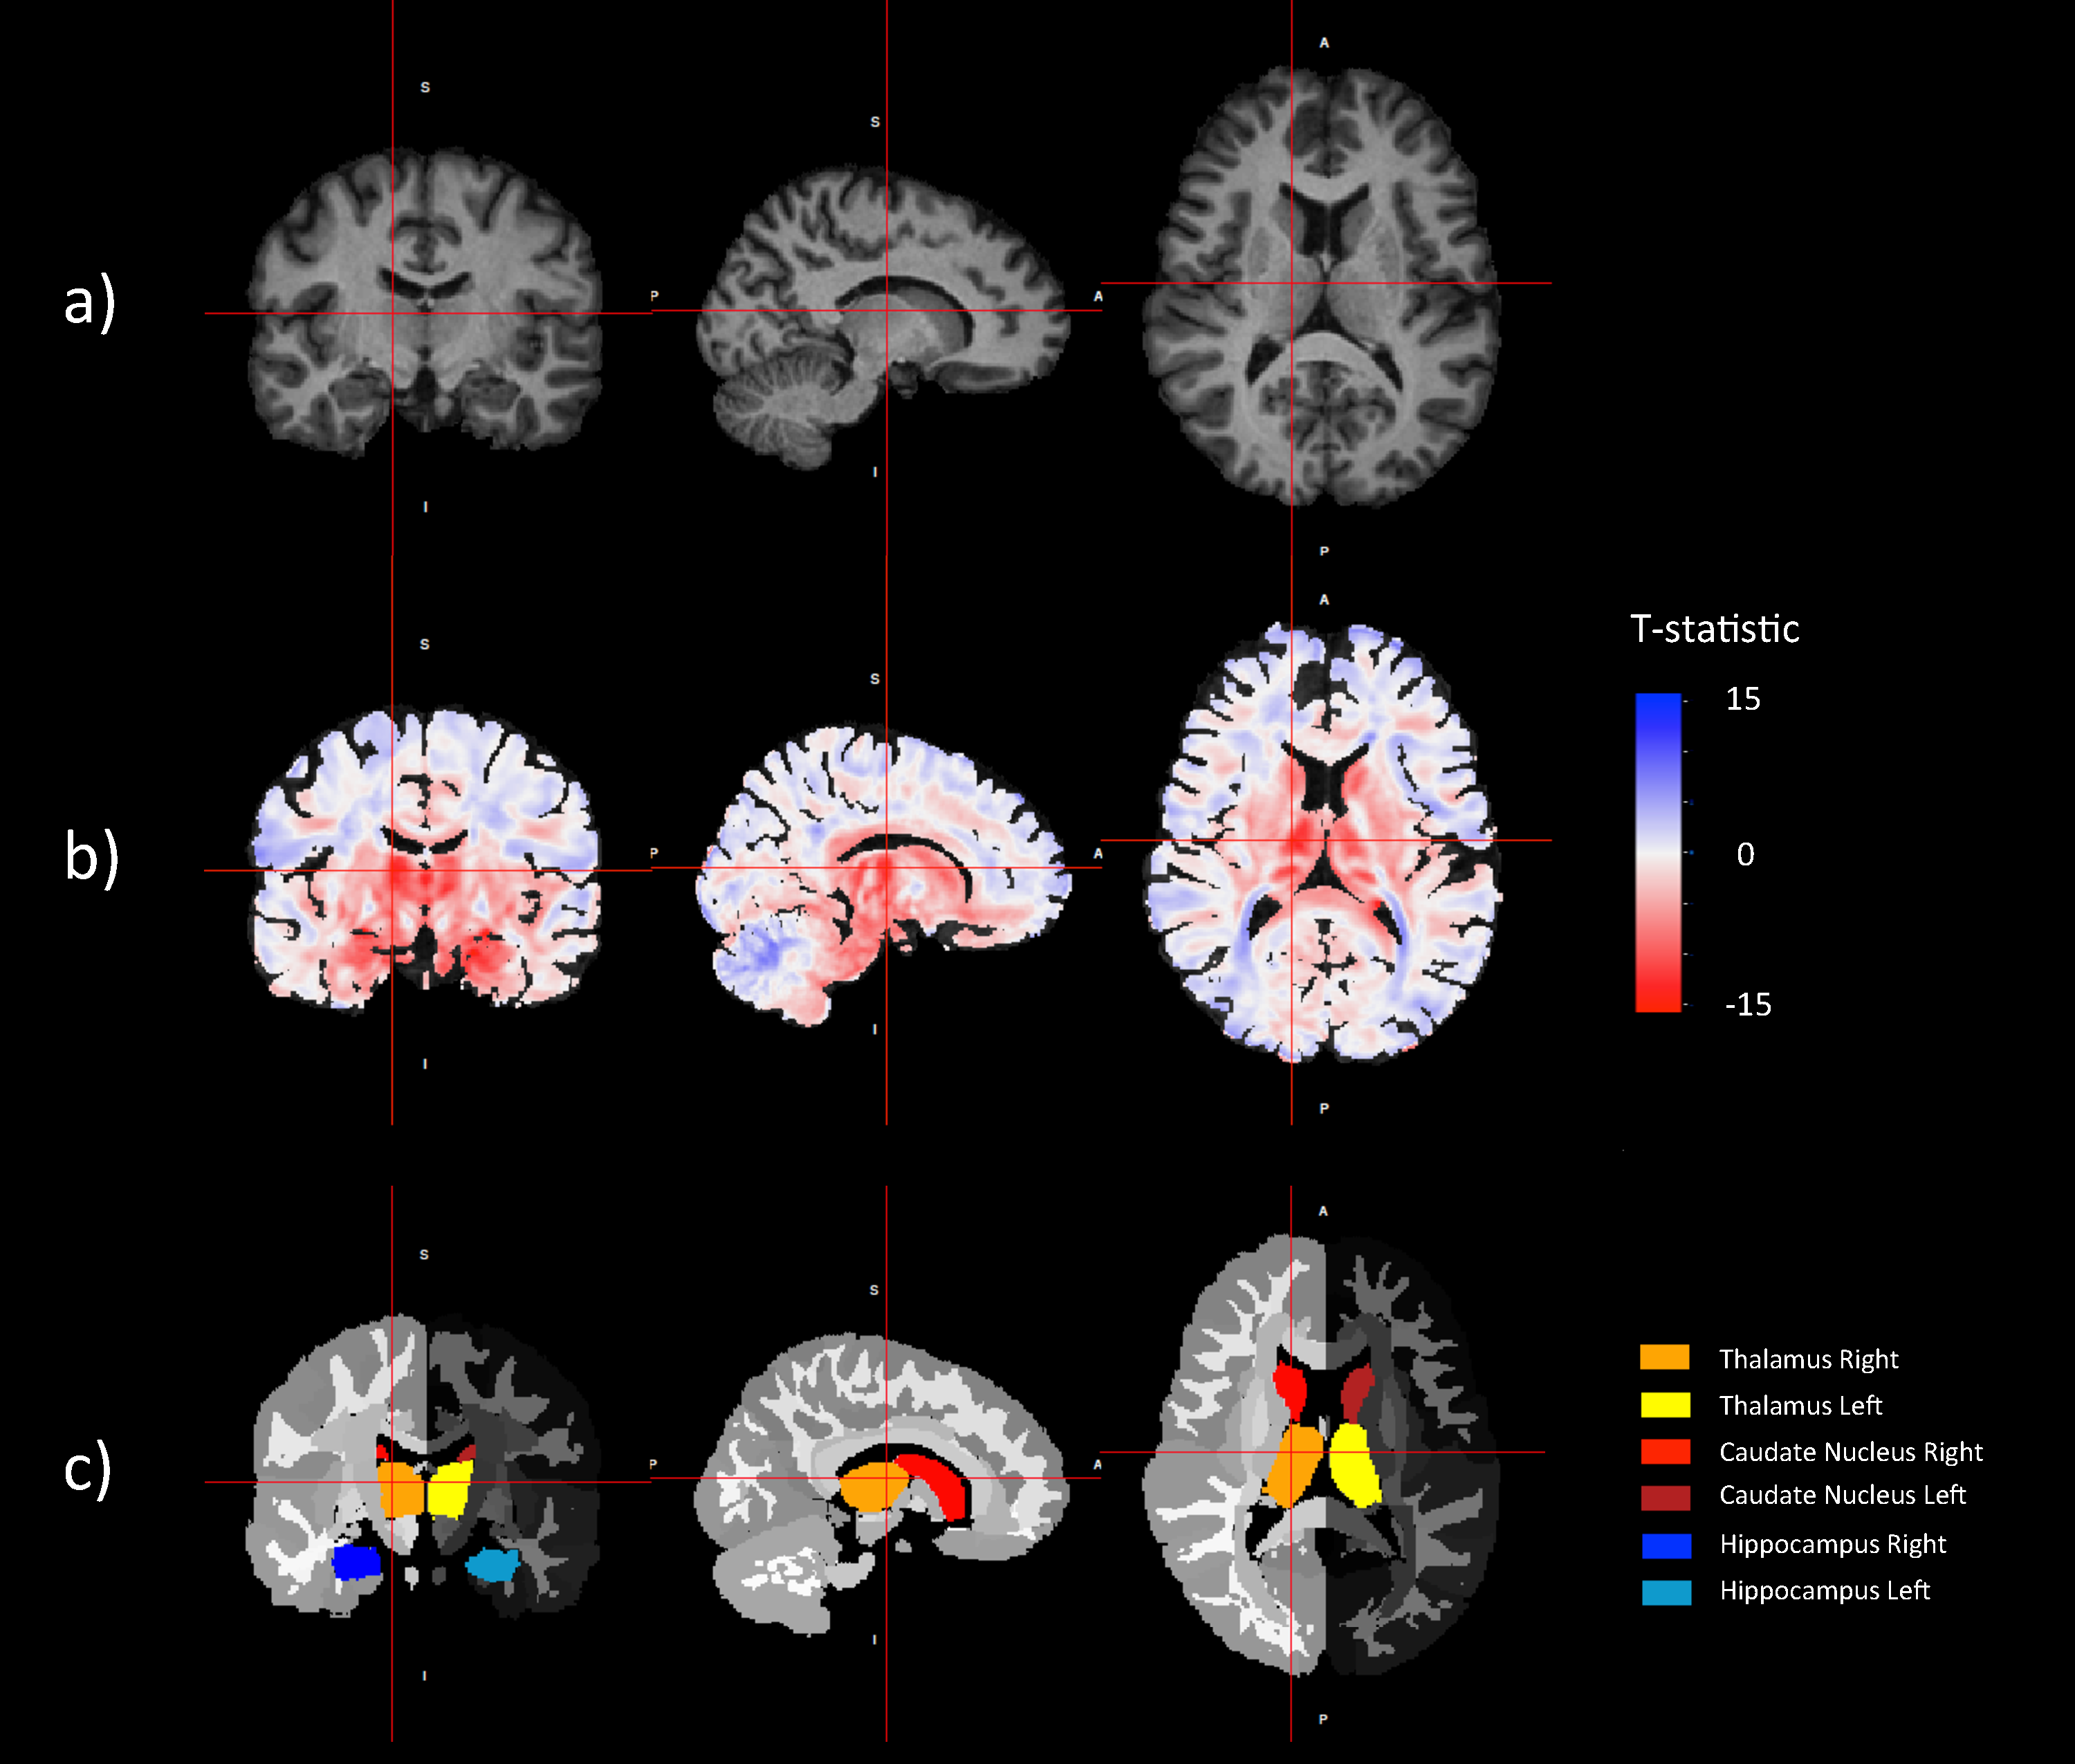
\includegraphics[height=5.5in]{figures/figure_dti.pdf}
    \label{fig:dti}
  \end{center}
\end{figure}

% Advanced data analysis and visualization}
\section{Advanced data analysis and visualization}
An important advantage  of the  {\rlang} environment  is that  more sophisticated voxel-level analyses can be easily implemented.  For  example, one could be interested  whether  there  are  additional confounders  for the association between FA and gender, or  whether  image intensities predict health outcomes. The \code{lm} and \code{glm} packages in {\rlang} are designed specifically to address such questions. If images are observed longitudinally or they are used as baseline predictors in longitudinal studies, one could use the mixed effects \pkg{gee} \cite{gee} and \pkg{lme4} \cite{lme4} packages. If one is interested in modeling survival time based on baseline images, then the \pkg{survival} package \citep{survival-package,survival-book} can be used. More advanced visualization of data and statistical results can be done using the packages \pkg{papayar}, which is an {\rlang} wrapper around \texttt{Papaya} \url{https://www.nitrc.org/projects/papaya/}, a \texttt{JavaScript} medical research image viewer. The \pkg{brainR} package in Neuroconductor is an {\rlang} only software for $3$D and $4$D visualization.

% Multi-site neuroimaging data harmonization
\section{Harmonization of multi-site neuroimaging data}\label{sec:datafusion}

An increasingly common strategy in Neuroimaging is to combine multi-site imaging data across scanners and protocols. This approach pools results from different sources and may improve statistical power to detect small effects  that would be undetectable in separate studies. However, the combination of multi-site data can introduce substantial unwanted variation in the data, due to differences in the scanner characteristics,  acquisition parameters, and preprocessing pipelines. This is highly problematic when this technical variability is larger than the biological variation of the phenotype of interest. We refer to the process of removing the technical variation in multi-site studies as ``harmonization''. 

The harmonization problem has long been recognized in genomics, where data across batches exhibit large technical variability. This technical variability is referred to in genomics as batch effects. When there is confounding between batch and phenotype, failing to account for batch effects can lead to spurious associations \citep{batchreview}. The development of several statistical batch effect correction tools in genomics has been under intense methodological development. This research has produced useful {\rlang} software packages that are deployed in Bioconductor and  are widely-used for the removal of batch effects. Some popular examples of such packages are  \texttt{ComBat} \citep{combat}, \texttt{SVA} \citep{sva1,sva2}, \texttt{RUV} \citep{ruv}, and limma \citep{limma1,limma2}. 

The Neuroconductor platform allows to integrate, adapt and extend these methods in imaging studies. For example, the \texttt{RUV} approach was adapted to structural MRI images and was shown to successfully remove technical variation in multi-site data from the Alzheimer's Disease Neuroimaging Initiative (ADNI). The methods are implemented in the Neuroconductor package \pkg{RAVEL} \citep{ravel}. 

% Data Packages
\section{Data Packages}\label{data-packages}
Neuroconductor hosts data packages that allow users to test
software or contain highly relevant data, such as templates. To be posted data need to be de-identified, the author/maintainer needs to have approval to make the data public, and all user agreements need to be respected. Neuroconductor also hosts packages that can access data from public repositories, while respecting the data user agreements.

%The developer perspective
\section{The developer perspective}\label{section:dev_perspective}

The comprehensive {\rlang} archive network (CRAN) is the most standardized, popular, and common way to distribute {\rlang} packages. Neuroconductor is complementary platform dedicated to developers of {\rlang} packages for image analysis that contains extensive specific training materials and includes packages that do not integrate directly with CRAN or may require additional checks with external dependencies.  The system is based on Git, GitHub, and continuous integration (CI) services via Travis CI.

Many developers use Git, a version control system, for their projects.  To distribute, host, and collaborate on  projects, many use online tools, with GitHub (\url{https://github.com/}) being one of the most popular.  As GitHub is an online site, distribution of a package can be done by downloading or cloning a repository.  Users can easily install {\rlang} packages directly from GitHub using functions from add-on {\rlang} packages, most notably \pkg{devtools} \cite{devtools}.  Along with a detailed and revertible timeline for each package, GitHub provides a page that allows users to flag issues for developers, metrics for package activity, and tag stable releases of the package.  Along with GitHub, the Travis CI (\url{https://travis-ci.org/}) provides a system to check packages as they are updated.  These tools provide a cloud-based infrastructure that: 1) can host and distribute packages; 2) check packages for specific requirements; 3) provide a platform for bug reporting and feature requests; and 4) check how frequently issues are addressed.

To submit a package, the author/maintainer of the package will have to provide their name, a valid email address and the GitHub URL for the package. A short description can also be added but it is not mandatory. Once the package is submitted several initial checks will be conducted; see Figure~\ref{fig:stage1} for details.

Once the verification is complete, the package will be processed according to the workflow described in Figure~\ref{fig:stage2}. 

Next, the package is pushed to the central Neuroconductor GitHub [\url{https://github.com/neuroconductor}] and submitted to Travis CI [\url{https://travis-ci.org/}] to be built and checked on multiple systems. The author of the package receives an automatic email indicating whether the package was built successfully and is integrated with Neuroconductor together with a description a file containing pertinent information about the process. The package author can ask for help from the maintainers of Neuroconductor [\url{https://neuroconductor.org/contact-us}] both for compatibility issues as well as for R-specific questions. 

\begin{figure}[!ht]
  \begin{center}
    \caption{Neuroconductor initial package submission stage. If the DESCRIPTION file is present it will parsed and the submitted version of the package is checked against existing Neuroconductor packages. If this version is not already in Neuroconductor the email based verification process is started. Once the maintainer verifies the submission the package is ready to be tested.}
    \label{fig:stage1}
    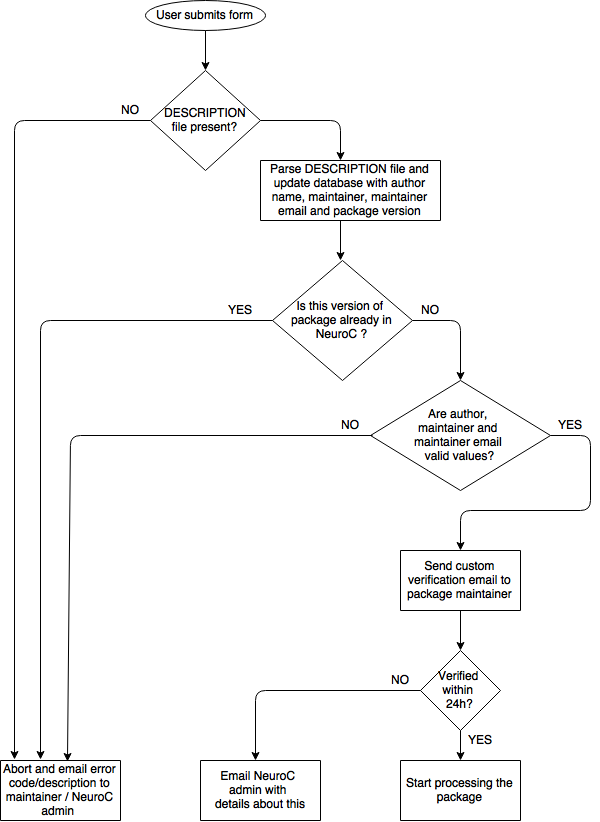
\includegraphics[height=0.9\textheight]{figures/flow_stage1_draft.png}\label{fig:package_lifetime_1}
% * <adig@jhu.edu> 2016-11-30T18:19:59.969Z:
%
% ^.
  \end{center}
\end{figure}
\begin{figure}[!ht]
  \begin{center}
    \caption{Neuroconductor package code testing. The package is cloned/updated on the Neuroconductor server and Travis CI checks are initiated for the original version of the package together with a stable and development version of this package. The DESCRIPTION and travis.yml files are updated to reflect the stable/development package status. Once the Travis CI checks are done the package listing is updated to reflect the check results.}
    \label{fig:stage2}
    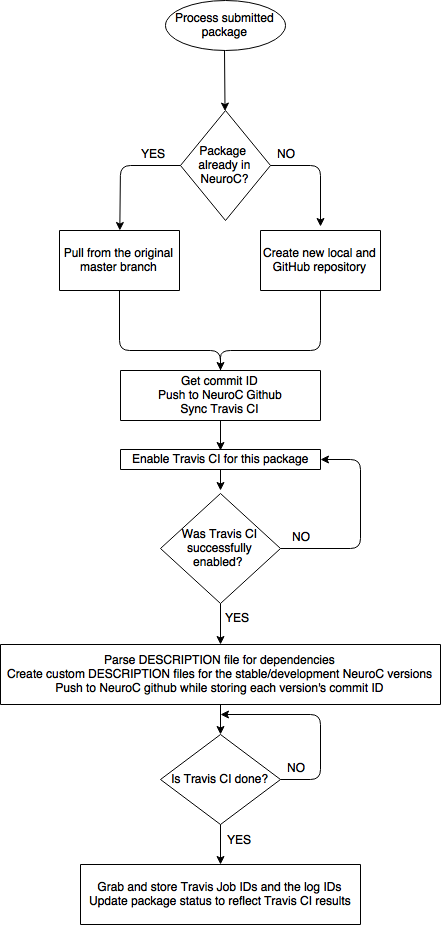
\includegraphics[height=0.9\textheight]{figures/flow_stage2_draft.png}\label{fig:package_lifetime_2}
  \end{center}
\end{figure}

%%%%%%%%%%%%%%%%%%%%%%%%%%%%%%%%%%%
% Table 
\begin{table}[!ht]
%\scriptsize
\centering
\caption{\textbf{Current R packages available on Neuroconductor}}\label{tab:packages}
\begin{tabular}{lll}
\hline \\[-2ex]
\textbf{Package} & \textbf{Description}   & \textbf{References} \\
\hline \\ [-1.5ex]
\multicolumn{3}{l}{\textbf{Software packages}}\\
\\ [-1.5ex]
\pkg{neurobase} & Base functions for Neuroconductor  &   \\
\pkg{oro.nifti} & Description  &  \citep{oro.nifti} \\
\pkg{oro.dicom} & Description  &  \citep{oro.nifti} \\
\pkg{oro.asl} & Description  &   \\
\pkg{oro.pet} & Description  &   \\
\pkg{ANTsR} & Advanced Normalization Tools  & \citep{ants} \\
\pkg{extrantsr} & Extensions for ANTsR  &  \\
\pkg{fslr} & R package for FSL  & \citep{fslr,fsl} \\
\pkg{freesurfer} & R package for FreeSurfer  & \citep{freesurfer} \\
\pkg{oasis} & OASIS lesion segmentation & \citep{oasis}\\
\pkg{WhiteStripe} & White Stripe intensity normalization  & \citep{whitestripe} \\
\pkg{RAVEL} & Statistical analysis of structural MRIs  & \citep{ravel} \\
\pkg{hcp} & R interface for the Human Connectome Project database &  \\
\hline \\ [-1.5ex]
\multicolumn{3}{l}{\textbf{Data packages}}\\
\\ [-1.5ex]
\pkg{kirby21.t1} &   & \citep{kirby}  \\
\pkg{kirby21.t2} &   &  \citep{kirby} \\
\pkg{kirby21.flair} &   &  \citep{kirby} \\
\pkg{kirby21.dti} &   &  \citep{kirby} \\
\pkg{kirby21.fmri} &   &  \citep{kirby} \\
\pkg{kirby21.mt} &   &  \citep{kirby} \\
\pkg{kirby21.vaso} &   &  \citep{kirby} \\
\pkg{kirby21.asl} &   &  \citep{kirby} \\
\hline \\ [-1.5ex]
\multicolumn{3}{l}{\textbf{Template packages}}\\
\\ [-1.5ex]
\pkg{MNITemplate} &   &   \\
\pkg{EveTemplate} & Eve Atlas and White Matter parcellation map  & \citep{eve}  \\
\end{tabular}
\end{table}




\bibliographystyle{plainnat}
\bibliography{Neuroconductor}

%\section*{References}\label{references}
%\addcontentsline{toc}{section}{References}
%
%\hypertarget{refs}{}
%\hypertarget{ref-carpux5fsecretux5f2012}{}
%Carp, Joshua. 2012. ``The Secret Lives of Experiments: Methods Reporting
%in the fMRI Literature.'' \emph{NeuroImage} 63 (1): 289--300.
%doi:\href{https://doi.org/10.1016/j.neuroimage.2012.07.004}{10.1016/j.neuroimage.2012.07.004}.
%
%\hypertarget{ref-gentleman2004bioconductor}{}
%Gentleman, Robert C, Vincent J Carey, Douglas M Bates, Ben Bolstad,
%Marcel Dettling, Sandrine Dudoit, Byron Ellis, et al. 2004.
%``Bioconductor: Open Software Development for Computational Biology and
%Bioinformatics.'' \emph{Genome Biology} 5 (10). BioMed Central: 1.

\end{document}


